\documentclass{article}[a4]
\usepackage[utf8]{inputenc}
\usepackage{authblk}
\usepackage{tabularx}
\usepackage{url}
\usepackage{verbatimbox}
\usepackage{graphicx}
\graphicspath{{images/}}

\title{Proposal of Automatic Extraction Framework of Superconductors related Information from Scientific literature}

\author[1]{Luca Foppiano\thanks{FOPPIANO.Luca@nims.go.jp}}
\author[1]{Thaer M. Dieb\thanks{MOUSTAFADIEB.Thaer@nims.go.jp}}
\author[1]{Akira Suzuki\thanks{SUZUKI.Akira3@nims.go.jp}}
\author[1]{Masashi Ishii\thanks{ISHII.Masashi@nims.go.jp}}
\affil[1]{Research and Services Division of Materials Data and Integrated System (MaDIS), National Institute for Materials Science (NIMS), 1-2-1 Sengen, Tsukuba, Ibaraki 305-0047, Japan}

% \date{April 2019}

\begin{document}

\maketitle

\begin{abstract}
Automatic collection of materials information from research papers using Natural Language Processing (NLP) is highly required for rapid materials development using big data, namely materials informatics (MI). Difficulty of this automatic collection is mainly caused by the variety of expressions in the papers, a system with tolerance to such variety is required to be developed. 
In this paper, we report an ongoing interdisciplinary work to construct the system for automatic collection of superconductor-related information from scientific literature using text mining techniques. 
We focus on identification of superconducting materials and their key property of critical temperature (Tc). We discuss the construction of a prototype for extraction and linking using machine learning (ML) techniques in order to define a baseline and a direction for future improvements.
\end{abstract}

%% The table of content is there just for organisation purposes, will be removed 
\pagebreak

% \tableofcontents

% \pagebreak

%Research in superconductors is always articulated over two main axes, finding new conditions or discovering new materials (or combination of it) show new or better superconductivity properties. 
%In order to do so, material scientists needs to have rapid access to materials known to be superconductors and their properties without have to examine the thousand of papers related to it. Such data can also be used by further systems to compute generative models 


\section{Introduction}
% What is the problem we are trying to solve? What are the motivation behind this project? 

Automatic extraction of information from research papers using Natural Language Processing (NLP) is a highly required approach in many domains. In material research, the utilisation of experimentally obtained big data may give insight leading to new breakthrough in materials discovery as known as Material Informatics (MI). Large availability of scientific papers and the expertise costs for manually extraction of valuable data justify the needs of Text and Data Mining (TDM) automatic approaches.
Despite the general understanding of necessity of TDM, variation in experiment and result descriptions make this task particularly complex. In this paper, we propose a framework for automatic data extraction and actual application of this system to a scientific filed, superconductivity.  

%% How research is made and what are the point of improvements?
\textit{Superconductivity is a phenomenon of exactly zero electrical resistance and expulsion of magnetic flux fields occurring in certain materials, called superconductors, when cooled below a characteristic critical temperature.}\footnote{\url{https://en.wikipedia.org/wiki/Superconductivity}}
Historically, high-temperature superconductors have been suddenly discovered by intuition of scientists rather than systematic consideration because of the lack of theoretical understanding \cite{klintenberg2013possible} \cite{DBLP:journals/corr/abs-1812-01995}. In this severe situation,  data-driven exploration \cite{doi:10.1080/14686996.2018.1548885}, \cite{HAMIDIEH2018346} \cite{PhysRevMaterials.2.024802} \cite{doi:10.1021/cm503507h} would be a feasible approach to accelerate development of new superconducting materials. Since it requires huge data sets for precise prediction, high-throughput experiments, first-principle calculations, existing material databases should be used as data source. Currently, several material databases are available for property search, however when looking at the superconductor sub-domain, the main one is SuperCon\cite{SuperCon} hosted and maintained by the National Institute for Materials Science (NIMS). Actually, the SuperCon contains about 32k inorganic and about 558 organic superconductor material definitions. Although it is still being updated manually, it cannot catch up with the massive fresh information from the increasing number of articles each year. It is our challenge to make SuperCon richer for data-driven science using TDM.

%The research in superconductor materials is articulated toward many different objectives. Discovery of new characteristic of well known materials, under new environment condition, like applied pressure or magnetic field. Combination of known superconductors with non-superconductors may lead to new materials with better characteristics, usually a higher critical temperature. 

% Add that introduction about the available databases, in particular NIMS, which has the problem that is not updated due to high costs of manual work
%Currently there are several general material databases available, however when looking  at the superconductor sub-domain the main one is SuperCon\cite{SuperCon}. Hosted and maintained by the National Institute for Materials Science (NIMS) containing about 32k inorganic and about 558 organic superconductor material definitions. Although the update continues manually, the latest information can not keep up with the increase in the enormous number of articles each year. 

% Why do we need such information? Why these information are important?
%The availability of material information with detailed and precise granularity is a must-have for superconductors scientists. This data summarises decades of research and discoveries and can be potentially exploited in many areas. Machine learning or neural models can train generative models specialised in automatically predict critical temperature \cite{DBLP:journals/corr/abs-1812-01995} on new (pure or intercalated) materials. Large scale repositories with enhanced search specialised in semantic superconductor disambiguation, document recommendation, and so on. 

In this paper we describe the ongoing attempt to design a TDM system using NLP techniques. In particular, we focus on extracting materials names and their linking with corresponding critical temperature (Tc) values.
Our system is built on an Open Source library for text mining from scholarly documents: Grobid \cite{GROBID}. We evaluate the performance of the system using precision, recall and f-score. Such preliminary results provides baseline for measuring our progress in solving the task.
Similar attempts of mining scientific literature in materials domain had been conducted \cite{nanocrystal_extraction} \cite{court2018auto}. 

% What we discuss in this paper? 
This paper is organised as follows, Section \ref{sec:architecture} describes the development of a working prototype specialised in superconductors data extraction including the development of an annotated corpus for material names recognition. Section \ref{sec:experiments-results} presents the evaluation methods and results, section \ref{sec:conclusion} concludes the paper.

\section{System architecture}
\label{sec:architecture}
The scientific information is often presented in tables and figures for quick understanding. However, in order to achieve higher order data structuring, it is necessary to link extracted entities. For example, the superconductor’s name with various expressions should be appropriately linked to corresponding property values depend on various parameters, such as dopant density, stoichiometry, and applied magnetic field. Obviously, these entities are not fully included in the tables and figures. Therefore, we insist on extracting information existing in the main body text and in captions of tables and figures. In superconductor sub-domain, since linking critical temperature (Tc) with its corresponding superconducting material is crucial, we constructed a system for the material and Tc (material-Tc) linking. Other properties will be targeted in the upcoming work.

We built our implementation based on an open source library called Grobid \cite{GROBID}. Grobid is a sequence labelling and document segmentation originally based on a Machine Learning algorithm Conditional Random Field (CRF) \cite{lafferty2001conditional}. It provides full support for extraction of data from PDF and a build-in workflow for pre-annotating training data, evaluation and training. 
The PDF support in Grobid was important because allowed us to work with a “standardised” medium instead of dealing with several flavour of XML formats. Among various available open source tools, the choice of Grobid is well justified by the fact that it's still actively developed and it's a production ready product deployed in the back-end of Mendeley \cite{mendeley-extraction} and other research repositories. Grobid performed best in a recent benchmark testing for citation extraction \cite{DBLP:journals/corr/abs-1802-01168}. Lastly, Grobid has been successfully extended to support several domains specific problems, for example astronomical entities recognition \cite{grobid-astro}, dictionaries segmentation \cite{khemakhem2017automatic}, software mention \cite{software-mentions} and measurements extraction and normalisation \cite{grobid-quantities}. The availability of an open source measurement recognition like Grobid-quantities was fitting perfectly for our use case to recognise Tc. 

\begin{figure}[]
    \centering
    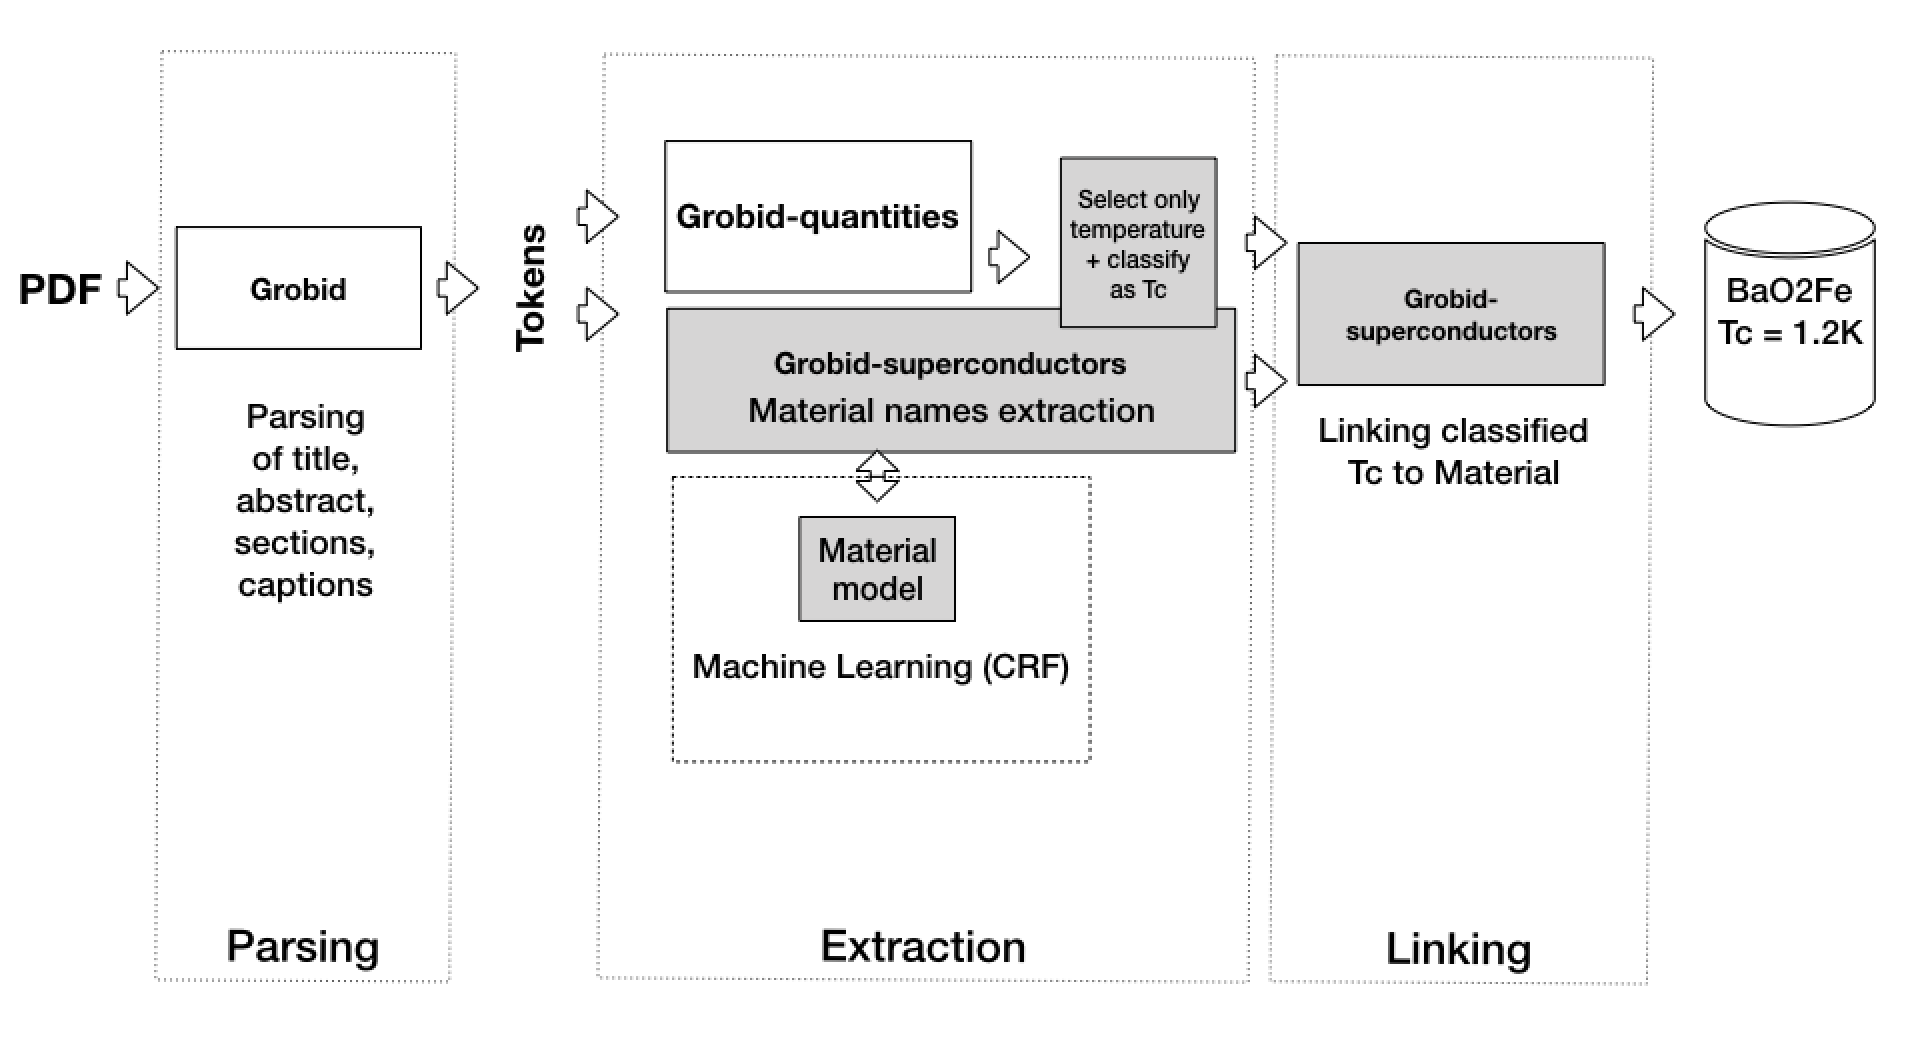
\includegraphics[width=4in]{schema}
    \caption[Schema of the system] {Schema of the system}
    \label{fig:system-schema}
\end{figure}

Our developed system illustrated in Figure \ref{fig:system-schema} consists mainly of two phases: “Extraction phase” and “Linking phase”. In the first phase, we extract relevant entities, i.e., superconducting materials and Tc, and in the second phase, we link these entities.

After parsing title, abstract, sections, and captions and following tokenisation, the Extraction phase combines the entities resulting from a newly trained model for superconductor material recognition and a conventional module, Grobid-quantities for measurement extraction. The superconductor material recognition model was trained with five full documents (forty two mentions in total) manually annotated. We added domain-specific features using a chemical recogniser, called ChemSpot \cite{10.1093/bioinformatics/bts183}. ChemSpot classifies the extracted entities into several classes: SYSTEMATIC, IDENTIFIER, FORMULA, TRIVIAL, ABBREVIATION, FAMILY, MULTIPLE and UNKNOWN.

In the following Linking phase, three tasks are performed: (1) since Grobid-quantities provides a larger set of measurements (temperatures, lengths, pressures, etc.) we selected only temperatures, then (2) we classified each of them into "Tc" and the others. Finally (3) we linked each material term with the closest Tc. 
The selection of Tc (2) was realised by word matching to an original dictionary, which summarises commonly used Tc-related words in superconducting literature (e.g. “Tc”, “critical temperature”). We looked for them in the surrounding of a numerical temperature assuming Tc related keywords will appear within five words. 
Finally the closest material term was linked to the pair of Tc and value, resulting in the entity linking of material-Tc-value. The linking interval was set to sentence or paragraph, we report results in the next section.
This simple algorithm allowed us to quickly develop a prototype implementing the end to end process and showing annotations directly in PDF or storing them in a database. In Figure \ref{fig:example-working} we show two examples of a correct linking, while in Figure \ref{fig:example-not-working} two example of incorrect linking or missing extraction. 

\begin{figure}[h]
    \centering
    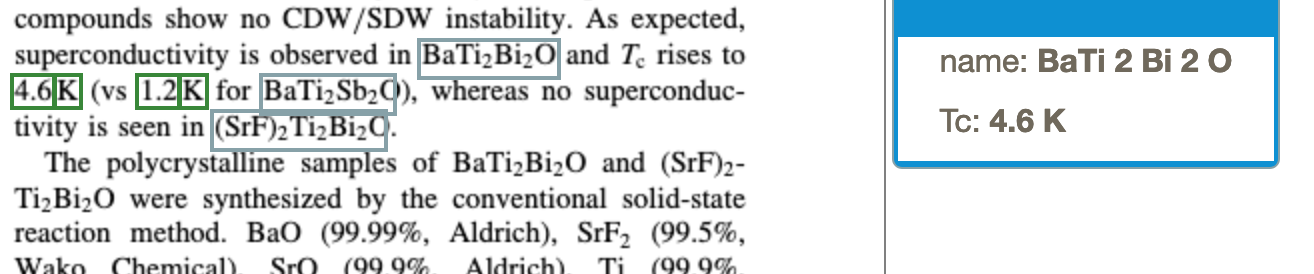
\includegraphics[width=4in]{example1} 
    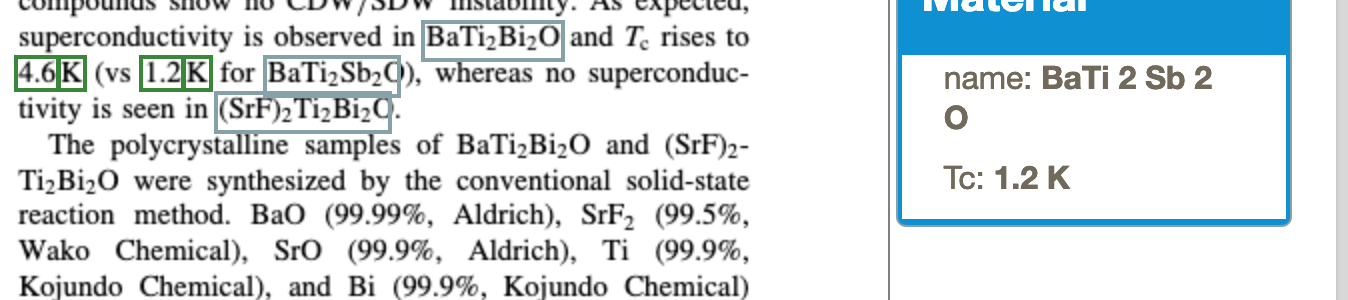
\includegraphics[width=4in]{example2}
    \caption{Example of a correct linking between material and Tc. The popup window indicate the links of material BaTi\textsubscript{2}Bi\textsubscript{2}O with Tc of 4.6K and BaTi\textsubscript{2}Sb\textsubscript{2}O with 1.2K}.
    \label{fig:example-working}
\end{figure}

\begin{figure}[h]
    \centering
    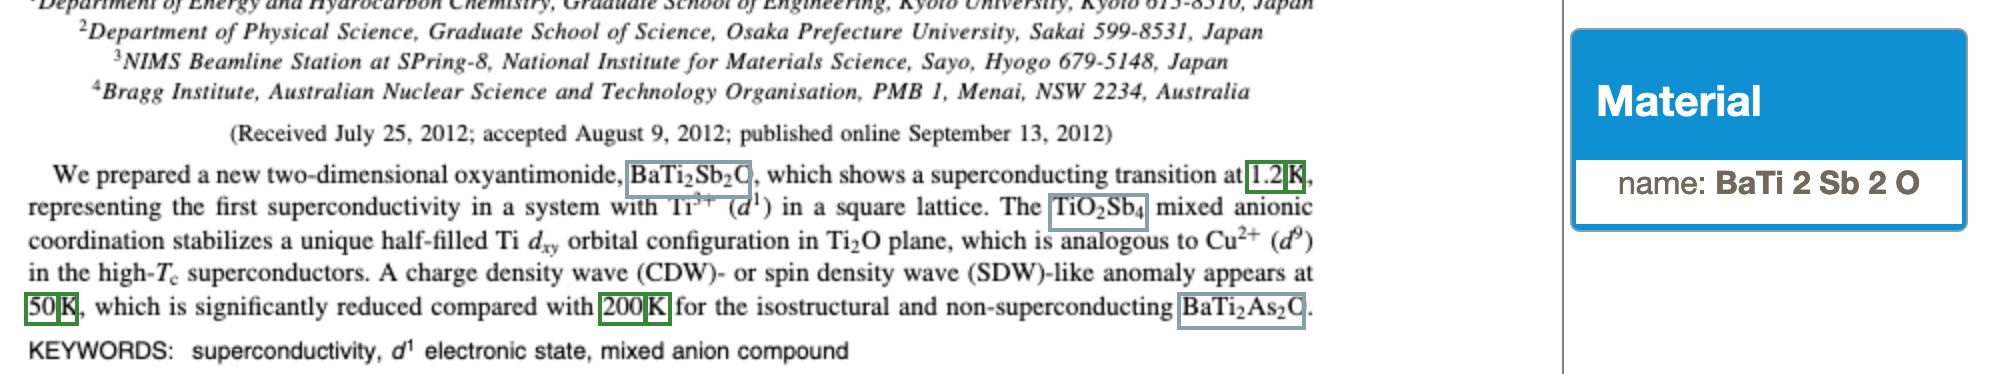
\includegraphics[width=4in]{example-bad1} 
    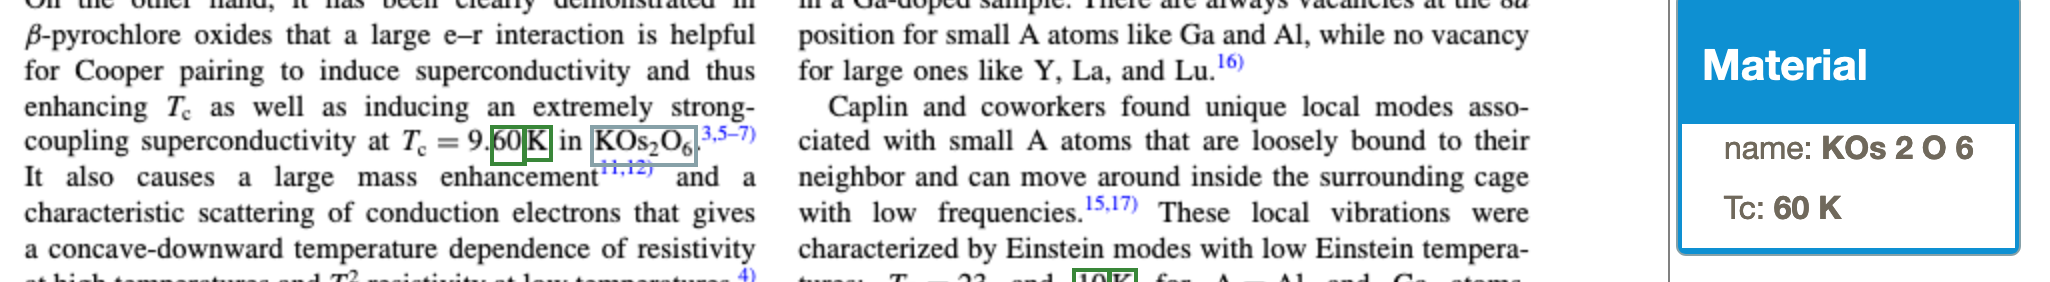
\includegraphics[width=4in]{example-bad2}
    \caption{Example of an incorrect linking between material and Tc. Although the material is correctly identified as BaTi\textsuperscript{2}Sb\textsuperscript{2}O, Tc is extracted incorrectly (correct Tc was 9.60 K while the extracted value was 60 K). }
    \label{fig:example-not-working}
\end{figure}

\section{Experiments and results}
\label{sec:experiments-results}

%In this section we evaluate the superconductor model trained with a small corpus and applied it to a larger corpus. 

The superconductor model was evaluated using a corpus of five papers (four for training and one for testing) having a total of forty-two entities classified with a single label called  \textless supercon\textgreater.

\begin{figure}[h!]
    \centering
    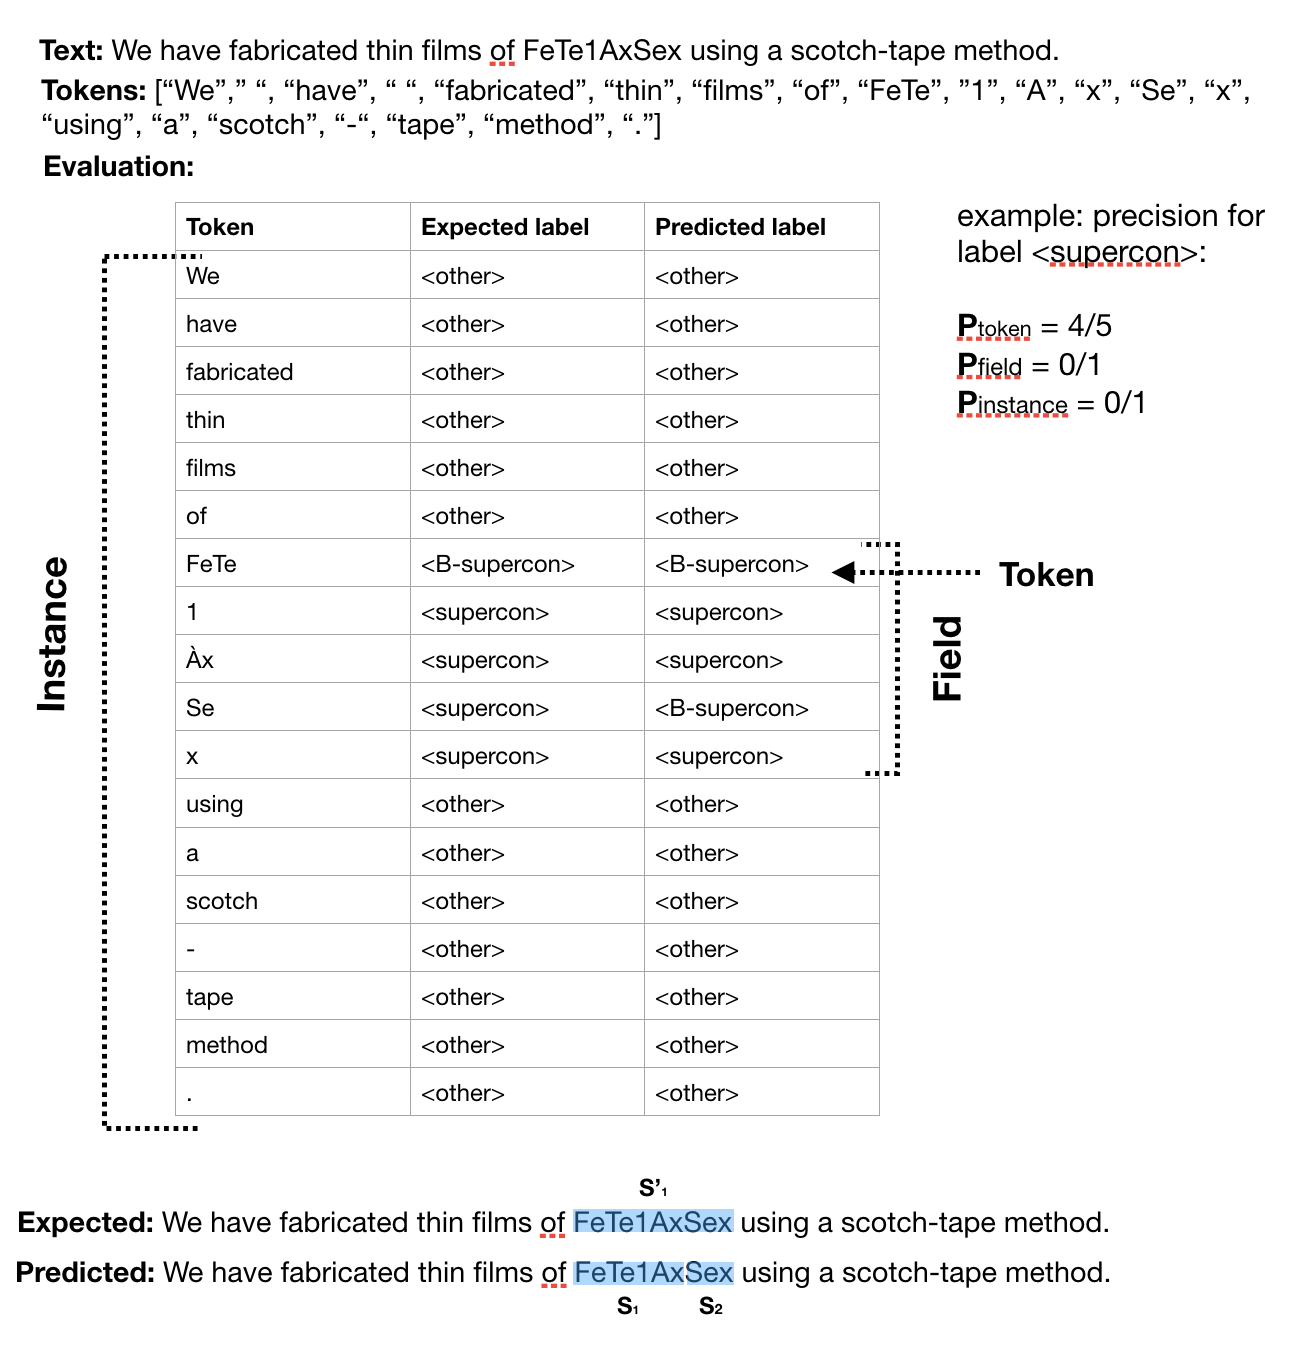
\includegraphics[width=4in]{example-output}
    \caption{Given a sentence (or paragraphs) the tokenisation transform it in an array of character sequences. These are then labelled by the ML CRF model. This figure illustrate the three different levels of granularity on which measurements are calculated.}
    \label{fig:levels-measurement}
\end{figure}

Grobid evaluation framework uses (accuracy, precision and recall) as evaluation measures. These measures are calculated at three different levels: tokens-level, field-level and instance-level. Figure \ref{fig:levels-measurement} illustrates the concept. 
Evaluation at token-level is computed considering each token independently (in the example we score 4/5), field-level consider each continuous sequence of the same label (a field, a sequence) belonging to the same labelled chunk (in the example  "FeTe\textsubscript{1}A\textsubscript{x}Se\textsubscript{x}" we score 0/1, because of a wrongly recognised token "Se"). Evaluation at instance-level is the score where all the entities within the same instance (a paragraph) must to be correct to consider the instance correctly recognised. 

Below is a snapshot of Grobid framework evaluation results: 

\begin{verbnobox}[\small]
===== Token-level results =====

label                accuracy     precision    recall       f1     

<supercon>           98.61        84.42        85.28        84.85  

all fields           98.61        84.42        85.28        84.85   (micro average)
                     98.61        84.42        85.28        84.85   (macro average)

===== Field-level results =====

label                accuracy     precision    recall       f1     

<supercon>           72.94        66.67        56.25        61.02  

all fields           72.94        66.67        56.25        61.02   (micro average)
                     72.94        66.67        56.25        61.02   (macro average)

===== Instance-level results =====

Total expected instances:   22
Correct instances:          15
Instance-level recall:      68.18
\end{verbnobox}

While token-level f-score was 84.85\%, the field-level f-score was 61.02\%. On the other hand, the recall at instance-level is 68.18\% indicating that the current training data have many paragraphs with no annotations. We conclude that such differences can be attributed to the lack of sufficient training data. 

Additionally, we tested the proposed system on a larger corpus of papers. We processed 500 PDF related to superconductors and evaluating the extracted critical temperatures and their link with the related material. 

In the Extraction phase (Table \ref{table:result-extraction}), in particular for material recognition we recorded mistakes at the boundaries of the annotation, for example LaFe\textsubscript{x}O\textsubscript{1-x} was extracted only as LaFexO missing the notation \textsubscript{2}. Other time two materials separated by "and" or a comma were extracted as a single entity. We are confident these mistakes will be reduced with more training data. Varieties of chemical compositions increase the number of the material entities. Temperatures could refer to experimental conditions or heat processes of specimen fabrication.

\begin{table}[h!]
    \centering
    \begin{tabular}{ | m{4em} | m{4em} | m{6em} | m{5em} | } 
    \hline
        Material entities & Unique material entities & Temperature entities & Tc entities \\
    \hline
        5400 & 1644 & 7554 & 1173 \\ 
    \hline
    \end{tabular}
    \label{table:result-extraction}
    \caption{Result of extraction of materials and critical temperatures from a corpus of 500 papers.}    
\end{table}

The results of the linking process (Table  \ref{table:result-linking}) showed extremely low (\textless 10/\%) recall. This is in line with the fact that Rule-Base approaches have tendency to be biased toward precision. 

We recorded precision using different boundaries to select the span of search for links to a specific material. Precision averaged around 68\% for sentence boundaries which was decreasing to 57\% using paragraph boundaries. 

\begin{table}[h!]
    \centering
    \begin{tabular}{ | c | m{5em}| m{5em}| m{5em}| } 
    \hline
        Boundaries & Links & Correct links & correctness  \\
    \hline
            sentences  & 112 & 77 & 68\% \\
    \hline
            paragraphs & 191 & 109 & 57\% \\
    \hline
    \end{tabular}
    \label{table:result-linking}
    \caption{Result of linking between materials and Tc.}    
\end{table}

Firstly, since we were processing PDFs we are aware the data in input contains noise like wrong UTF-8 characters, stream ordering issues, missing fonts, etc. Intuitively, Rule-based approach don't perform particularly well with noisy data, 
 
We assume that, the availability of more training data might leverage the system performance.

\section{Conclusion}
\label{sec:conclusion}
In this paper, we proposed an automatic extraction of superconductor related information from related scientific publications. The proposed system consists of two steps: a Machine Learning sequence labelling process for entity extraction and a simple rule-base for linking. 

We report that using Sequence labelling was promising; however increasing the size of the corpus is crucial for performance improvement. On the other hand, the experiment in linking using Rule-Based, thanks to variability of expressions, noise introduced and the different ways of describing experiments suggests to take a different approach exploiting the probability model and Machine Learning abilities. 

In the next step, we plan to test deep neural networks like Bi-LSTM+CRF approach and embedding for the extraction phase. 
Additionally, we would like to explore more probabilistic approaches like sequence labelling for linking entities within the same sentence in order to overcome the noisy data problem.

\pagebreak

\bibliography{references}
\bibliographystyle{plain}

\end{document}
